% !TEX program = pdflatex
% Rapport Séances 3 & 4 + CDC à jour — HireLink · EL ASSAL Douae
\documentclass[11pt,a4paper,oneside]{report}

\usepackage[T1]{fontenc}
\usepackage[utf8]{inputenc}
\usepackage[french]{babel}
\usepackage{geometry}
\geometry{left=2.4cm,right=2.2cm,top=2.3cm,bottom=2.5cm,headheight=14pt}
\usepackage{graphicx}
\graphicspath{{assets/}}
\usepackage{xcolor}
\usepackage{setspace}
\onehalfspacing
\usepackage{titlesec}
\titleformat{\chapter}[display]{\normalfont\huge\bfseries\color{burgundy}}{\chaptertitlename\ \thechapter}{10pt}{\Huge}
\titleformat{\section}{\normalfont\Large\bfseries\color{burgundy}}{\thesection}{0.7em}{}
\titleformat{\subsection}{\normalfont\large\bfseries}{\thesubsection}{0.5em}{}
\usepackage{fancyhdr}
\pagestyle{fancy}
\fancyhf{}
\fancyhead[L]{\small\textit{HireLink --- Séances 3 \& 4}}
\fancyhead[R]{\small\thepage}
\fancyfoot[C]{\footnotesize ENSA Tétouan · Frameworks Technologie Web · 2025--2026}
\renewcommand{\headrulewidth}{0.4pt}
\usepackage{amsmath}
\usepackage{booktabs}
\usepackage{array}
\usepackage{tabularx}
\usepackage{longtable}
\usepackage{enumitem}
\usepackage{tcolorbox}
\tcbuselibrary{skins,breakable}
\usepackage{hyperref}
\hypersetup{colorlinks=true,linkcolor=burgundy!80!black,urlcolor=burgundy,citecolor=burgundy}
\usepackage{float}
\usepackage{caption}
\captionsetup{font=small,labelfont=bf}

\definecolor{burgundy}{RGB}{122,32,50}
\definecolor{ink}{RGB}{26,18,20}
\definecolor{soft}{RGB}{247,241,234}

\newtcolorbox{reqbox}[1][]{
  colback=soft,colframe=burgundy,boxrule=0.7pt,arc=2pt,
  left=8pt,right=8pt,top=6pt,bottom=6pt,#1
}
\newtcolorbox{okbox}{
  colback=green!4,colframe=burgundy!70!black,boxrule=0.5pt,arc=2pt,
  left=6pt,right=6pt,top=4pt,bottom=4pt
}

\newcommand{\logo}[2]{%
  \IfFileExists{assets/#1}{\includegraphics[height=#2]{assets/#1}}{\fbox{\scriptsize #1}}%
}

\begin{document}

%==============================================================================
\begin{titlepage}
\centering
\vspace*{0.3cm}
{\large\bfseries UNIVERSITÉ ABDELMALEK ESSAÂDI}\\[2pt]
{\normalsize École Nationale des Sciences Appliquées de Tétouan}\\[12pt]
\begin{minipage}{0.3\textwidth}\centering\logo{logo-uae.png}{1.7cm}\end{minipage}\hfill
\begin{minipage}{0.3\textwidth}\centering\logo{logo-hirelink.png}{1.5cm}\end{minipage}\hfill
\begin{minipage}{0.3\textwidth}\centering\logo{logo-ensa.png}{1.7cm}\end{minipage}
\vspace{1cm}
\rule{\linewidth}{1.2pt}\\[8pt]
{\LARGE\bfseries\color{burgundy} Rapport de livraison}\\[4pt]
{\Large Séances 3 \& 4 --- Modélisation JPA et CRUD REST}\\[6pt]
{\huge\bfseries\color{burgundy} HireLink}\\[4pt]
{\large Plateforme ATS de recrutement (candidat · recruteur · admin)}\\[6pt]
{\normalsize\textit{Mise à jour du cahier des charges · Diagramme de classes · Réponses aux requis}}\\[8pt]
\rule{\linewidth}{1.2pt}
\vspace{0.9cm}
\begin{tabular}{@{}ll@{}}
\textbf{Étudiante} & Douae EL ASSAL \\
\textbf{Formation} & GI3 --- ENSA Tétouan \\
\textbf{Module} & Frameworks Technologie Web \\
\textbf{Stack} & Spring Boot 3 · Java · JPA/Hibernate · MySQL · HTML/JS \\
\textbf{API} & \texttt{http://127.0.0.1:8081/api/v1} \\
\textbf{Frontend} & \texttt{http://127.0.0.1:5500} \\
\textbf{Base} & \texttt{hirelink} (MariaDB / phpMyAdmin) \\
\textbf{Date} & octobre 2026 \\
\end{tabular}
\vfill
{\small Ce document aligne le cahier des charges et les livrables S3/S4 sur l'état réel de l'application.}
\end{titlepage}

\tableofcontents
\newpage

%==============================================================================
\chapter{Cahier des charges --- version actualisée}

\section{Contexte et problème}
HireLink n'est pas un simple jobboard. C'est un \textbf{ATS} (Applicant Tracking System) qui orchestre le cycle de sélection après candidature : pipeline d'étapes, délai de première réponse affiché (SLA), motifs de refus documentés, matching compétences, scorecard, et vérification d'entreprise avant publication.

Trois refus du marché motivent le produit :
\begin{itemize}[leftmargin=1.2em]
  \item offres sans engagement de délai de réponse ;
  \item refus sans motif exploitable ;
  \item entreprises non authentifiées qui publiquent librement.
\end{itemize}

\section{Acteurs}
\begin{tabularx}{\textwidth}{@{}lX@{}}
\toprule
\textbf{Acteur} & \textbf{Rôle dans HireLink} \\
\midrule
Candidat & Dépose un CV, complète le profil, consulte offres et entreprises, postule, suit ses dossiers, utilise la synthèse CV (crédits). \\
Recruteur & Crée une organisation (ICE), obtient un badge (auto ou admin), publie des offres, gère le pipeline, invite l'équipe. \\
Administrateur & Suit les stats, vérifie les entreprises en attente, gère plans / comptes / motifs de refus. \\
\bottomrule
\end{tabularx}

\section{Fonctionnalités livrées (état actuel de l'app)}
\subsection{Espace candidat}
\begin{itemize}[leftmargin=1.2em]
  \item Tableau de bord (profil, score CV, prévisualisation CV, offres recommandées, Premium).
  \item Offres (liste / détail), entreprises avec logo et badge, mes candidatures.
  \item Paramètres : Profil, Parcours, Image (sans photo stockée), CV, alertes ; formule \textbf{Essentiel} / \textbf{Performance}.
  \item Topbar : Passer Premium · cloche notifications · icône profil.
  \item Police UI : \textbf{Inter} ; palette bordeaux HireLink.
\end{itemize}

\subsection{Espace recruteur}
\begin{itemize}[leftmargin=1.2em]
  \item Dashboard, pipeline (SLA), CRUD offres, fiche entreprise (ICE, logo, relancer vérification), paramètres / Premium.
  \item Publication bloquée si l'entreprise n'est pas vérifiée.
\end{itemize}

\subsection{Espace admin}
\begin{itemize}[leftmargin=1.2em]
  \item Stats, file « à vérifier », bouton Vérifier / Retirer, plans, comptes.
\end{itemize}

\subsection{Sécurité et confiance}
\begin{itemize}[leftmargin=1.2em]
  \item Auth : e-mail + mot de passe, OTP à l'inscription, Google Sign-In.
  \item Vérification entreprise hybride (ICE + e-mail pro $\rightarrow$ auto ; sinon revue admin).
  \item JWT ; rôles \texttt{CANDIDAT}, \texttt{RECRUTEUR}, \texttt{ADMINISTRATEUR}.
\end{itemize}

\section{Règles métier clés}
\begin{reqbox}
\begin{enumerate}[leftmargin=1.4em]
  \item Inscription libre $\neq$ publication libre : badge entreprise obligatoire pour publier.
  \item Chaque offre affiche un délai de 1\textsuperscript{re} réponse (SLA).
  \item Un refus documenté s'appuie sur le catalogue de motifs.
  \item L'IA (synthèse CV) assiste ; elle ne postule ni ne décide.
  \item Essentiel candidat : 5 synthèses CV / mois ; Performance : sans plafond.
\end{enumerate}
\end{reqbox}

\section{Évolutions par rapport aux versions CDC antérieures}
\begin{tabularx}{\textwidth}{@{}>{\bfseries}p{3.2cm}X@{}}
\toprule
Point & Mise à jour \\
\midrule
UX candidat & Alignée sur une expérience type Stagiaires (dashboard 3 colonnes, entreprises, candidatures split). \\
Organisation & Champs logo, site, secteur, ville, présentation, \texttt{verificationMethod}. \\
Vérification & Automatique (registre ICE) + file admin ; API \texttt{/organizations/public}, \texttt{/mine/verify}. \\
Typographie & Inter pour toute l'UI. \\
Formules & Performance / Premium décrites (bénéfices, prix, retour possible). \\
\bottomrule
\end{tabularx}

%==============================================================================
\chapter{Architecture et modèle de données}

\section{Architecture en couches}
\[
\text{Frontend HTML/JS} \;\xrightarrow{\text{JWT}}\; \text{Controller} \;\rightarrow\; \text{Service} \;\rightarrow\; \text{Repository JPA} \;\rightarrow\; \text{MySQL \texttt{hirelink}}
\]
La source de vérité du schéma est le modèle Java (\texttt{@Entity}). Hibernate applique \texttt{ddl-auto=update} au démarrage. phpMyAdmin sert à contrôler, pas à inventer le schéma.

\section{Diagramme de classes (état actuel)}
\begin{figure}[H]
\centering
\IfFileExists{assets/diagramme_classes.png}{%
  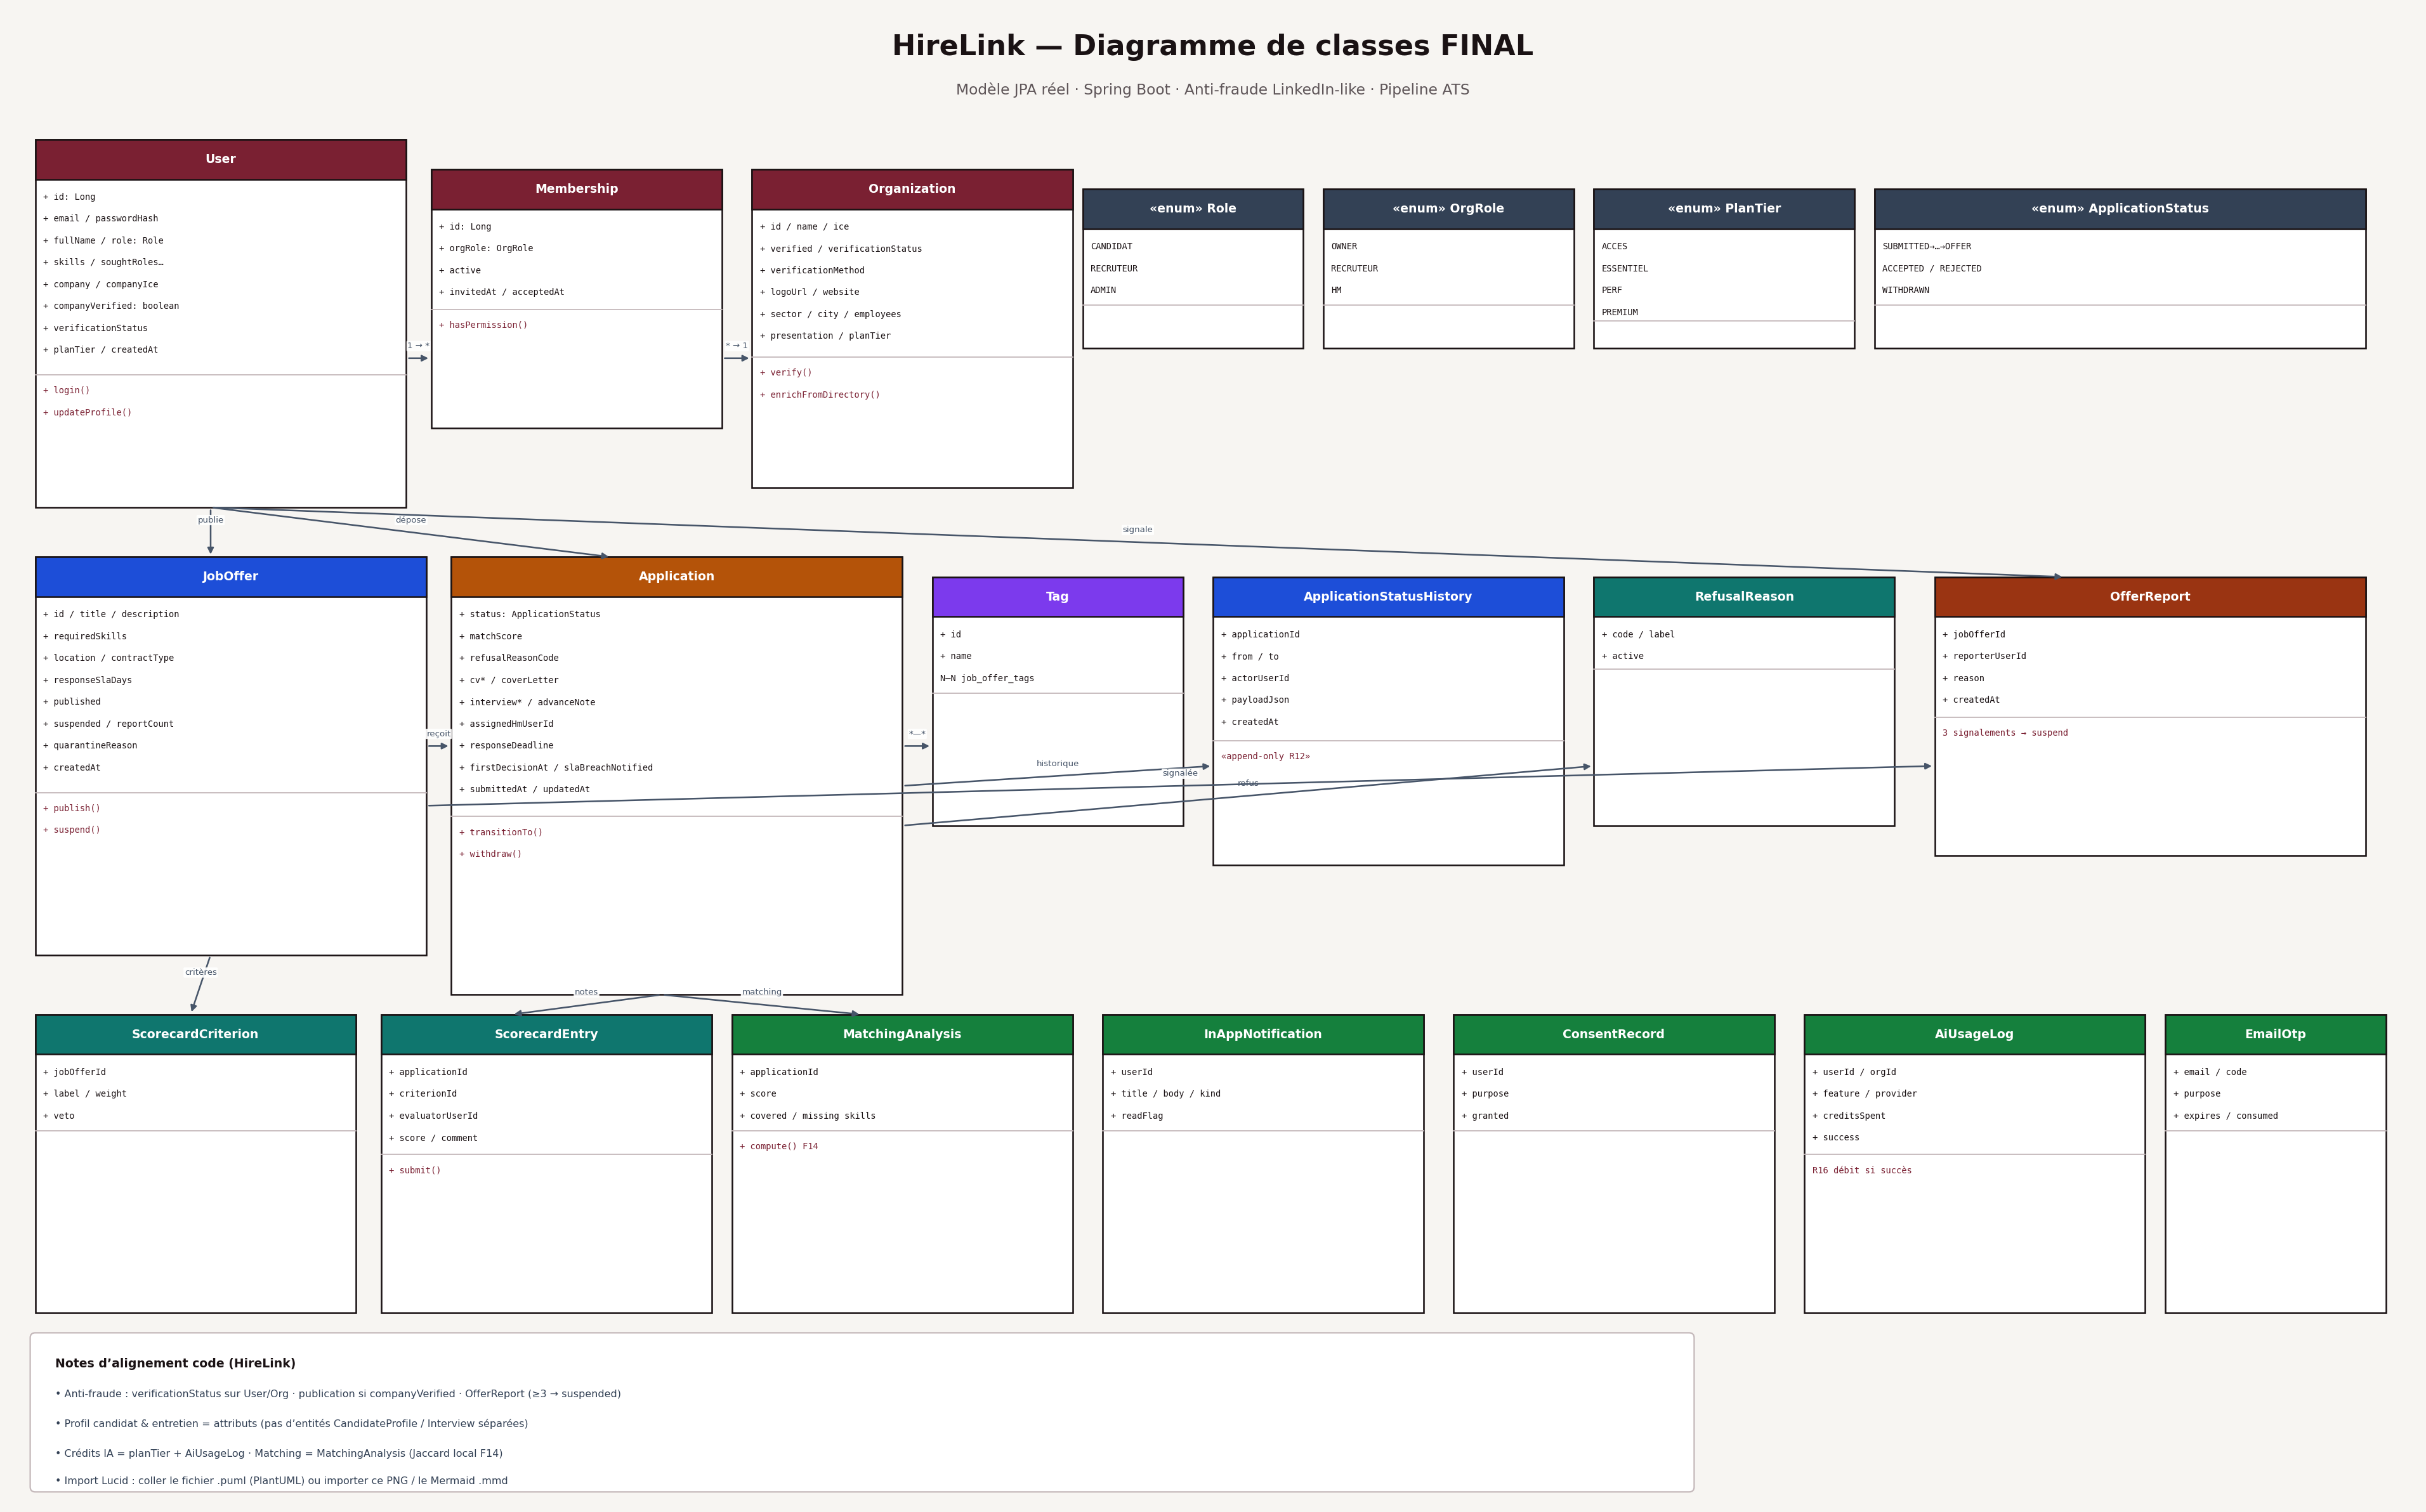
\includegraphics[width=\textwidth]{assets/diagramme_classes.png}%
}{\fbox{\parbox{0.9\textwidth}{\centering Diagramme manquant --- régénérer via \texttt{\_gen\_classes\_final.py}}}}
\caption{Diagramme de classes HireLink (JPA réel : User, Organization, Membership, JobOffer, Application, Tag, Notification, Scorecard, Matching, vérif entreprise, etc.).}
\label{fig:classes}
\end{figure}

\section{Entités et tables}
\begin{tabularx}{\textwidth}{@{}llX@{}}
\toprule
\textbf{Entité} & \textbf{Table} & \textbf{Rôle} \\
\midrule
User & users & Comptes, profil, CV, ICE, plan \\
Organization & organizations & Entreprise, badge, logo, plan \\
Membership & memberships & Lien User$\leftrightarrow$Org + OrgRole \\
JobOffer & job\_offers & Offres + SLA + quarantine \\
Application & applications & Candidatures + statut pipeline \\
Tag & tags / job\_offer\_tags & Tags ManyToMany \\
RefusalReason & refusal\_reason\_catalog & Motifs de refus \\
InAppNotification & notifications & Cloche in-app \\
MatchingAnalysis & matching\_analyses & Scores matching \\
Scorecard* & scorecard\_* & Évaluation multi-critères \\
AiUsageLog & ai\_usage\_logs & Crédits / synthèse CV \\
\bottomrule
\end{tabularx}

\section{Relations JPA principales}
\begin{itemize}[leftmargin=1.2em]
  \item User (recruteur) $1$---$*$ JobOffer ; User (candidat) $1$---$*$ Application.
  \item JobOffer $1$---$*$ Application.
  \item User $\leftrightarrow$ Organization via Membership (association avec attributs OWNER / RECRUTEUR / HIRING\_MANAGER).
  \item JobOffer $\leftrightarrow$ Tag : \texttt{@ManyToMany}.
  \item Organization $\rightarrow$ User (owner) : \texttt{@ManyToOne}.
\end{itemize}

%==============================================================================
\chapter{Ce que nous avons réalisé}

\section{Séance 3 --- Modélisation JPA / Hibernate}
\begin{enumerate}[leftmargin=1.4em]
  \item Identification des entités à partir du CDC ATS.
  \item Annotations \texttt{@Entity}, enums (\texttt{Role}, \texttt{OrgRole}, \texttt{ApplicationStatus}, \texttt{PlanTier}).
  \item Mapping des relations (ci-dessus).
  \item Configuration datasource \texttt{127.0.0.1:3306/hirelink} + \texttt{ddl-auto=update}.
  \item Contrôle phpMyAdmin + diagramme de classes livré.
  \item Formulaires frontend alignés (profil, offres, pipeline, entreprise).
\end{enumerate}

\section{Séance 4 --- CRUD et API REST}
Trois CRUD complets démontrés :

\begin{tabularx}{\textwidth}{@{}lX@{}}
\toprule
\textbf{Entité} & \textbf{Endpoints} \\
\midrule
JobOffer & POST/GET/PUT/DELETE \texttt{/api/v1/offers} (+ \texttt{/mine}, \texttt{/public}) \\
RefusalReason & CRUD \texttt{/api/v1/refusal-reasons} (admin) \\
InAppNotification & CRUD + \texttt{/\{id\}/read} \texttt{/api/v1/notifications} \\
\bottomrule
\end{tabularx}

Preuves : UI \texttt{recruiter-offers.html}, \texttt{admin-refusal-reasons.html}, cloche ; collection Postman \texttt{docs/postman/HireLink\_CRUD\_Seance4.postman\_collection.json}.

\section{Compléments livrés (hors « 3 CRUD » mais cohérents)}
Auth (OTP / Google / complete-profile), pipeline candidatures, organisations (vérif + logos publics), admin entreprises, CV multipart + synthèse \texttt{/ai/cv-summary}, marketplace d'offres seedées.

\section{Score CV, synthèse et vérification (clarifications produit)}
\subsection{Score CV}
Calcul côté frontend sur les \textbf{sections} du CV : Identité /15, Expériences /25, Formation /20, Compétences /25, Langues /15. Seuils : A $\ge 80$, B $\ge 55$, sinon C. Ce n'est pas de l'IA.

\subsection{Analyse vs synthèse}
L'analyse (onglets) est une checklist automatique. La synthèse (\texttt{POST /ai/cv-summary}) produit un texte court à partir des sections ; elle consomme un crédit Essentiel (5/mois) et est journalisée dans \texttt{ai\_usage\_logs}.

\subsection{Vérification entreprise}
ICE + nom + e-mail professionnel $\rightarrow$ badge automatique si registre OK ; sinon file admin. Sans badge : publication refusée.

%==============================================================================
\chapter{Réponses aux requis --- Séance 3}

\begin{reqbox}[title=\textbf{Requis Séance 3}]
Construire le modèle de données et le relier au backend : entités JPA, relations, Hibernate, MySQL, diagramme de classes, formulaires alignés.
\end{reqbox}

\begin{okbox}
\textbf{Réponse --- statut : SATISFAIT}
\begin{enumerate}[leftmargin=1.3em]
  \item \textbf{Entités JPA} : package \texttt{ma.ensat.hirelink.model} (User, Organization, Membership, JobOffer, Application, Tag, RefusalReason, InAppNotification, Scorecard, Matching, etc.).
  \item \textbf{Relations} : \texttt{@ManyToOne}/\texttt{@OneToMany}, Membership N--N, \texttt{@ManyToMany} JobOffer$\leftrightarrow$Tag.
  \item \textbf{Hibernate} : \texttt{spring.jpa.hibernate.ddl-auto=update} --- tables créées/mises à jour au démarrage Spring Boot (pas de \texttt{schema.sql} comme source de vérité).
  \item \textbf{MySQL} : schéma \texttt{hirelink} visible dans phpMyAdmin (\texttt{http://127.0.0.1/phpmyadmin/}).
  \item \textbf{Diagramme de classes} : figure~\ref{fig:classes} et fichiers \texttt{docs/diagrammes/diagramme\_classes\_hirelink\_FINAL.*}.
  \item \textbf{Formulaires} : pages candidat / recruteur / admin branchées sur les champs persistés.
\end{enumerate}
\end{okbox}

\textbf{Compétences couvertes :} JPA, Hibernate, ORM, mapping objet-relationnel, relations, persistance.

%==============================================================================
\chapter{Réponses aux requis --- Séance 4}

\begin{reqbox}[title=\textbf{Requis Séance 4}]
Développer un CRUD complet sur au moins trois entités, exposer une API REST, préparer les interfaces frontend, tester avec Postman.
\end{reqbox}

\begin{okbox}
\textbf{Réponse --- statut : SATISFAIT}
\begin{enumerate}[leftmargin=1.3em]
  \item \textbf{CRUD 1 --- JobOffer} : Controller \texttt{/api/v1/offers} + Service + Repository ; UI recruteur créer / modifier / supprimer ; gate entreprise vérifiée.
  \item \textbf{CRUD 2 --- RefusalReason} : endpoints admin ; UI \texttt{admin-refusal-reasons.html}.
  \item \textbf{CRUD 3 --- InAppNotification} : create / list / mark-read / delete ; cloche dans la topbar.
  \item \textbf{Architecture} : Controller $\rightarrow$ Service $\rightarrow$ Repository $\rightarrow$ Entity (démontrable ligne par ligne).
  \item \textbf{Frontend} : \texttt{fetch} + JWT (\texttt{frontend/js/api.js}) vers \texttt{http://127.0.0.1:8081/api/v1}.
  \item \textbf{Postman} : collection officielle dans \texttt{docs/postman/} (login JWT puis scénarios CRUD).
\end{enumerate}
\end{okbox}

\textbf{Compétences couvertes :} Spring Data, Repository, Service, REST Controller, CRUD HTTP, manipulation de données.

\section*{Tableau récapitulatif « demandé / livré »}
\begin{tabularx}{\textwidth}{@{}p{4.2cm}X@{}}
\toprule
\textbf{Demande} & \textbf{Livré} \\
\midrule
Modèle JPA + relations & Entities + Membership + ManyToMany Tags \\
Hibernate $\rightarrow$ MySQL & \texttt{ddl-auto=update}, base \texttt{hirelink} \\
Diagramme de classes & PNG + PlantUML + figure dans ce rapport \\
CRUD $\ge$ 3 entités & Offres, Motifs, Notifications \\
API REST & Controllers \texttt{/api/v1/**} \\
UI + Postman & Pages app + collection Postman \\
\bottomrule
\end{tabularx}

%==============================================================================
\chapter{Annexes}

\section{Comptes de démonstration}
\begin{itemize}[leftmargin=1.2em]
  \item Admin : \texttt{admin@hirelink.ma} / \texttt{Admin123!}
  \item Recruteur : \texttt{n.bennani@atlasdigital.ma} / \texttt{Recruteur123!}
  \item Candidat : \texttt{candidat@hirelink.ma} / \texttt{Candidat123!}
\end{itemize}

\section{Démarrage rapide}
\begin{enumerate}[leftmargin=1.3em]
  \item XAMPP : MySQL + Apache (phpMyAdmin).
  \item Backend : \texttt{mvn spring-boot:run} dans \texttt{backend/} (port 8081).
  \item Frontend : \texttt{python -m http.server 5500} dans \texttt{frontend/}.
  \item Santé : \texttt{GET /api/v1/health} $\rightarrow$ UP + \texttt{catalog=hirelink}.
\end{enumerate}

\section{Chemins utiles}
\begin{verbatim}
HireLink/
  backend/src/main/java/ma/ensat/hirelink/{model,repository,service,controller}
  frontend/app/
  docs/diagrammes/diagramme_classes_hirelink_FINAL.png
  docs/postman/HireLink_CRUD_Seance4.postman_collection.json
  docs/cahier-des-charges/
  docs/livraison-seance3-4/rapport-latex/   ← sources de ce PDF
\end{verbatim}

\section{Conclusion}
Les objectifs des séances 3 et 4 sont \textbf{atteints} : modèle JPA cohérent avec le métier ATS, schéma MySQL généré par Hibernate, CRUD REST démontrable, UI et Postman. Le cahier des charges et le diagramme de classes de ce document reflètent l'\textbf{état actuel} de HireLink (vérification entreprise, logos, UX candidat, formules, Inter).

\end{document}
